\chapter{Texte aus der Vorbereitung}

\section{Ein Spionagebericht}
{\itshape
Diese Berichte scheinen Helme Haffax, Azaril Scharlachkraut, Arngrimm von Ehrenstein, und Travian von Rabenmund zu beschreiben.
}

``Wie steht es um das Südheer?'', fragt der große Mann in den Raum. Fackeln erleuchten ihn nur schwach und das unregelmäßige Licht wirft große Schatten an die steinernen Wände. Der hagere Magier erblasst, das Licht lässt ihn wie verhungert erscheinen: “D.. die G.. Gotongis sind in die 7. Sphäre zurück gefahren, Herr. Wir haben keine Informationen über das Verbleiben der Obristin von Perricums oder ihres Generalsstabs. Wir, wir müssen davon ausgehen, dass das alle magischen und exsphärischen Einheiten des Verbandes vernichtet wurden.” Er reibt nervös seine Hände und blickt sich um. Die anderen Gestalten im Raum bleiben regungslos und starren zurück, ihre Mienen verraten nichts. Kaum merklich nickt der große Mann und der Magier eilt aus dem Raum \dots

\dots In einem Schankraum, in einer düsteren Ecke sitzt eine wunderschöne Frau. Ihr edles Kleid, ihr hochnäsiger Blick und ihr vorsichtig geschminktes Gesicht machen deutlich, dass sie von Stand ist und doch sitzt sie ohne Begleitung oder Eskorte in einer Taverne. Die Atmosphäre ist gedrückt, das Licht erhellt den späten Abend nur schwach. Die Namenlosen Tage verbringt niemand gerne außerhalb der eigenen vier Wände.

Ein Schatten fällt auf die Frau und ihr maskenhaftes Gesicht verzieht sich zu einem dünnen Lächeln. Sie nickt zu dem freien Stuhl neben sich und dabei wird ein Blick auf ihre Ohren frei, auf spitze Ohren. “Habt ihr euch an die neuen Umstände gewöhnt?” fragt sie den Neuankömmling, eine Gestalt, die komplett durch einen langen schwarzen Mantel verhüllt ist. „Ja“, gibt dieser zurück und setzt sich . „Seid ihr sicher, dass sie kommen werden?“, fragt er langsam, als müssten sich seine Lippen noch an die Worte gewöhnen. Eine silberhelles Lachen ertönt, doch es klingt wie eine Glocke auf einem Boronsanger, „Wo sollen sie denn sonst hingehen“, fragt die Frau und blickt den dunklen Mann direkt an. ``Sie werden kommen, das verspreche ich euch, und wir werden auf sie warten...'' \dots

\dots Zwei Männer reiten über ein Schlachtfeld, um sie herum ertönt das Stöhnen der Verwundeten und die Schreie derer, die mehr gesehen haben, als sie sollten. Die beiden Männer scheinen das nicht zu bemerken, sie blicken auf die brennende Burg vor ihnen. Sie sehen sich sehr ähnlich, in ihrem prunkvollen silbernen Rüstungen, die die Zeichen der Schlacht tragen. Auf ihren Schildern prangen ein Wolf und ein Rabe und ihre Klingen sind noch rot vom frischen Blut vieler toter Soldaten.

``Die Thronräuber und Verräter fliehen wie die Ratten vor dem Feuer!'', meint der Jüngere mit dem Rabenwappen triumphierend, und richtet seinen Blick auf den Älteren neben ihm ``Bald werden wir vor den Mauern Wehrheims stehen und dann werden sie wissen, dass eine neue Ära angebrochen ist!'' Der Ältere blickt weiter grimmig auf das flammende Inferno und meint: ``Die Verräter und Ursupatoren werden büßen, für das was uns genommen wurde! Und das schon bald!'' Plötzlich wendet er seinen Kopf zu seinem Gefährten und fährt dann bestimmt fort: ``Du wirst verlangt.'' Der Rabenritter blickt ihn überrascht an und antwortet mit fester Stimme: ``Was immer ihr befiehlt, Herr, ich bin euer gehorsamster Diener!'' ``Es wird eine Jagd geben und die Legatin des Meisters verlangt einen Bluthund.'' Unterwürfig verneigt sich der Jüngere: ``Ich bin bereit für die Hatz.'' ``Folge dem Heer. Ihr werdet euch bald treffen. Und das Wild wird dir ganz besonders gefallen...'' \dots

\section{Die Trümmer von Kurkum}

Die Trümmer der mächtigen Wehrmauern und Gebäude Kurkums ragen schwarz vor Ruß in den Himmel auf. Die Luft riecht nach Rauch und Asche, das Knacken von schwelenden Balken dringt an euer Ohr. Das Tal ist still, tot, nach dem Lärm der Schlacht. Leises Schluchzen erklingt, eine alte Frau stöhnt verzweifelt als die Überlebenden den Tempel der Rondra verlassen. Wie ein Stück einer anderen Welt steht der Leuentempel da, wie eine Erinnerung an eine vergangene Zeit, unberührt von Schlacht ud Flammenmeer. Vielen um euch herum kullern Tränen über die Wangen und hinterlassen Furchen in dreckigen Gesichtern. Der beißende Geruch nach Rauch, der heiße Staub, all das lässt auch eure Augen tränen. Das stoze Volk der Amazonen, die hehren Soldatinnen der Rondra sind in die Hallen des Mythraelsfeldes eingegangen.

Rohana von Kurkum, die letzte Kriegerin der Feste, tritt zwischen euch. Ihr Harnisch ist verbeult und ihre Kleidung von Blut durchtränkt. Sie trägt einen tiefen Schnitt über ihre linke Wange und humpelt ein wenig. In ihrem bleichen Gesicht zeichnet sich Verzweiflung ab und in ihren kraftlosen Fingern hält sie ein zerbrochenes Schwert. Unter dem Dreck und der Asche erkennt ihr einen kunstvoll gearbeiteten Griff. Es ist das Schwert der Königin, zerbrochen durch den letzten Schlag des furchtbaren Dämons.

``Geht hinaus!'' flüstert sie mit letzter Kraft, ``Verkündet der Welt, dass Yppolita von Kurkum gefallen ist! Das Kurkum gefallen ist!''

\chapter{Ausarbeitung der Baronie}

{\itshape
Lieber Waldemar,

Ich habe hier einige Aufzeichnungen zusammen getragen, die einst die Chronik der Baronie hätten werden sollen. Ich hoffe, sie sind als Kontext für die Berichte der Gezeichneten nützlich.
}

\section{Grunewaldt: Geschichte}

Grunewaldt, ehemals Ebersberg, ist eine kleine Baronie im westlichen Tobrien. Nachdem der alte Verweser des Grafen, Baron von Stahlheim zu Ebersberg, seine Befugnisse überschritten und die Region maßlos ausgebeutet hat, eroberte der junge Jasper von Grunewaldt, ein Edler der Region, die Baronie und schlug den Söldnerhaufen des Stahlheimers. Der Edle wurde in der wirren Kaiserlosen Zeit von Graf Rondradan von Streitzig als Herrscher von Grunewaldt eingesetzt. Um den Göttern für die Wendung des Schicksals der Baronie zu danken beschloss der junge Jasper dem Praios eine Siegeskirche zu bauen. Diese Kirche verschlingt nun schon seit mehreren Jahren Unsummen, und langsam beginnen die Bauern der Region unmütig zu raunen.

Nach dem tragischen Tod des Jasper von Grunewaldt bei der Jagd, fiel die ertragreiche Baronie an den Herrn zurück, da der verblichene keine Kinder hinterließ. Um Schulden beim Herzog von Tobrien auszugleichen, beschloss von Streitzig, diesem die Baronie zu vermachen, ein Entschluss, der ihm einiges an Überwindung abverlangte. Die Baronie wurde einem jungen Sprössling des Hauses Ehrenstein, Arngrimm dem Jüngeren als Lehen verliehen, der sich sofort an eine weitere Ausbeute der Minen und einen Ausbau der wirtschaftlichen Vormachtstellung machte. Viele der älteren Bewohner nahmen dies nicht gut auf; sie waren skeptisch wegen der großen Träume ihres Herren. Die jüngeren aber träumten genau wie Arngrimm von einer Heimat, die man in einem Zuge mit Ysilia, Warunk und Mendena nennen würde. Das bis dahin der Weg noch sehr weit war, ignorierten viele fröhlich.

Nach Arngrimms vorzeitigem Ableben beim Scharmützel von Tuzak war die Baronie wieder herrenlos und wurde von Ratsherr Eichmannsson im Name des Herzogs von Tobrien regiert. Nach der Rettung des Herzogs Bernfried in der Schlacht von Vierreichen, wegen der großen Verdienste um das Herzogtum in den Schlachten von Kurkum, Eslamsbrück und Vierreichen und wegen der Beschaffung der Hauer des Mendenischen Ebers erhob der Herzog den Edlen Ragnos vom Svelltal zu Klammsbrück in den Rang eines Barons zu Grunewaldt. Er sollte die Bewohne seiner neuen Baronie in die letzte Schlacht gegen den Dämonenmeister führen.

\section{Grunewaldt: Land und Leute}

Die Nähe der schwarzen Sichel mit ihren Silberminen und Steinbrüchen macht die Baronie einigermaßen ertragreich, obwohl sie inmitten einer armen Region liegt. Der Norden der Baronie ist größtenteils bewaldet und versumpft, der Süden hingegen ist zur landwirtschaftlichen Nutzung geeignet. Hier wird ein Großteil des Korns der Baronie geerntet. Die Minen im Westen brachten lange nur wenig ein. Während der kurzen Herrschaftszeit Arngrimms des Jüngeren von Ehrenstein wurden diese Minen jedoch deutlich vergrößert so dass kurz vor dem Tobrienkrieg der Handel zu florieren begann. 

Die Baronie hat drei größere Städte: Grunewaldt (ehem. Ebersberg), mit 530 Einwohnern die größte und wichtigste Stadt, Kornheim, mit 350 Bürgern das Getreidezentrum im Süden und Stahlheim, ehemals 600 Einwohner, heute noch etwa 200, der ehemalige Hauptsitz der Barone.

\section{Die Stadt Grunewaldt}
Die Stadt Grunewaldt ist die Hauptstadt der Baronie und zeigt dies auch offen und stolz. Durch Handel und Friede ist die Stadt sehr wohlhabend geworden und nennt sich trotz praktisch fehlendem Stadtrecht: Stadt. Das ist auch das Ziel dieser kleinen und kämpferischen Gemeinde. Aber man ist dem Herrscher Jasper trotzdem nicht abgeneigt gewesen, die Kleinbürger waren durchaus stolz, dass „ihr“ Edler die Baronskrone errungen hat. Auf den neuen Verwalter der Baronie blickt man mit typischer konservativer Skepsis, ist einer Neuerung aber nicht grundsätzlich abgeneigt.

Auf dem Weg zum Stadtrecht haben die Städter sich eine eigene „Verwaltung“ und die Befreiung aus der Leibeigenschaft erkämpft. Grunewaldt ist sozusagen Stadt mit dem Baron als Stadtherrn.

Wichtige Orte der Stadt sind der Marktplatz und die Burg. Dort befinden sich eigentlich alle wichtigen Gebäude. Einige Gewerbe und Handwerker haben sich dort niedergelassen. So findet sich dort das „Große Handelshaus und Lager“ welches für den Handel mit Silber und Stein zuständig ist und bescheidenen Reichtum erwirtschaftet hat. Auch ein Silberschmied und Schmuckmacher, weit über die Grenzen der Baronie hinaus berühmt hat hier seine Werkstadt, nebenbei ist er am äußerst lukrativen Silberhandel beteiligt.

\subsection{Gebäude und wichtige Orte der Stadt}

Das Garnisionshaus, welches ein größeres Haus nahe der Stadtmauer ist, bietet den Stadtbütteln einen Platz zum Schlafen, Gefängniszellen zum Festhalten von auffällig gewordenen Bürger und einen ausreichend großen Innenhof, der als Übungsplatz für die Büttel dient. Die meisten Büttel sind jedoch für ein ausreichend großes Handgeld bereit ein Auge zuzudrücken. 

\subsection{Tobimorahafen}
Der 25 Schritt lange seitlich in den Fluss hinein gebaute Holzdock mit dazugehörigem steinernem Hafenhäuschen, den die Bewohner liebevoll Hafen nennen, bietet kleinen Flussschiffen eine Anlegestelle für die Nacht und die Möglichkeit ihre Waren zu löschen und neue aufzunehmen. Da die Tobimora hier nur einen Bruchteil so groß ist, wie weiter unten an der Mündung bei Mendena, ist der Handel über den Fluss auch von geringerer Bedeutung, da größere Flusssegler können hier nicht anlegen können und somit nur der Transport von kleinen Warenmengen möglich ist. Und überhaupt trauen sich nur erfahrene Flussschiffer zu, die Stromschnellen bis zur nächsten größeren Stadt Ebelried zu meistern. Der Hafen liegt nicht innerhalb der Stadtmauern. Doch allein die Tatsache einen Tobimorahafen zu besitzen, steigert das Ansehen der Stadt gewaltig. Im kleinen Hafenhäuschen sitzt der Hafenverwalter Eberhard Karjensen zusammen mit den Handelsaufzeichnungen der letzten zehn Götterläufe und führt Buch über die eingehenden und ausgehenden Waren, sowie über die Zollabgaben. Er ist ein kauziger alter(60) Kerl, der die Handelsregister des Hafens beinahe auswendig kennt. Die zum Hafen zugehörigen Lagerhäuser stehen innerhalb der Stadtmauer.

\subsection{Marktplatz \& Händler}
Gleich mehrere reiche Händler haben sich am Marktplatz angesiedelt und verkaufen dort ihre Waren. Unter anderem der überregional bekannte Silberhändler, ein Steinhändler und ein Holzhändler.

Alle vier Wochen in den Sommermonaten findet hier ein überregionaler Markt für Güter aller Art statt, auf dem sowohl die Waldbauern, die nur selten in die Stadt finden, als auch alle Händler aus der Stadt, sowie vorbei reisende Händler ihre Waren anbieten.

\subsection{Tempel und Schreine}
\paragraph{Praioskathedrale}
Die Praioskathedrale wird als Siegeskirche für den Sieg der Grunewalder über die Stahlheimer gebaut und wurde vom alten Baron Jasper von Grunewaldtin Auftrag gegeben. Doch auch nach vielen Jahren Bauzeit steht zurzeit nur das Grundfundament und mit den nicht sehr üppigen Geldspritzen des Barons wird sich das nicht so schnell ändern. Doch dank des Bauvorhabens sind immer ein paar Priester des Praios, sowie ein paar Bannstrahler in der Stadt.   

\paragraph{Perainetempel}
Der Perainetempel ist die feste Vertretung der Perainekirche in der Region. Er liegt ein wenig entfernt vom Marktplatz, zwischen diesem und dem Stadttor. Tatsächlich lassen sich die meisten Perainegeweihten jedoch auf den Feldern im Süden der Stadt finden, wo sie den Bauern bei der Arbeit helfen und die Felder segnen. Doch auch wenn man mit einer Verletzung, einer Krankheit oder einem anderen Anliegen in den Tempel kommt, wird einem geholfen. Meist kümmert sich die alte Tempelvorsteherin Treunai Jolen von Reiherweiher um einen gleich persönlich, meistens beobachtet von mindestens einem der Novizen des Tempels. Mit ihrer freundlichen, unaufgeregten und beruhigenden Art ist sie sehr beliebt bei ihren Patienten. Dank ihres Alters hat sie viel Erfahrung, ist jedoch körperlich nicht mehr in der Lage lange auf dem Feld zu arbeiten. 

\paragraph{Boronschrein}
Der kleine Boronschrein liegt zwar innerhalb der Stadtmauern, jedoch in guter Laufnähe zum Boronsanger, der außerhalb der Stadt liegt. Er wird vom alten Borongeweihten Anshag Kohlmoor betreut, der auf seine alten Tage sein Leben der Erhaltung des Tempels und des Boronsangers gewidmet hat. Auf seine alten Tage hört er und sieht er nicht mehr gut und spricht mit kratziger Stimme. Sein Geist ist jedoch noch scharf. Er lebt von den Spenden der Bewohner. 

\paragraph{Firunsschrein}
Der Firunsschrein wird vom Jäger des Barons betreut. Er ist auch für die Opfer für den eisigen Gott verantwortlich. Nur selten kommt ein Firunsgeweihter vorbei um selbst Opferrituale abzuhalten. Der Firunsschrein ist direkt an der Stadtmauer gelegen und karg gehalten. Nur eine Statue aus Stein ziert den Schrein.

\paragraph{Ingerimmsschrein}
Der Ingerimmsschrein steht direkt neben der örtlichen Schmiede, denn er wird auch vom örtlichen Schmied und seinen Lehrlingen geführt. Wie bei den anderen Schreinen kommt ein Geweihter nur alle paar Monde vorbei.

\subsection{Die Burg des Barons}
Die Burg des Barons von Grunewaldtliegt verschiedenen Berichten zufolge gleichzeitig direkt neben der Stadt Grunewald, von zwei kleinen Flüssen eingerahmt und nahezu uneinnehmbar vom Fluss aus und nur schwer einnehmbar von der Stadt aus oder wahlweise auf einem der Hügel der Umgebung auch hier schwer befestigt aufgrund der Streitigkeiten mit den Stahlheimern. Die Burg ist nicht groß. Platz genug im Haupthaus für den Baron und seine Dienerschaft, die nicht sehr groß ist, einen kleinen Stall, einen Trutzturm, einen Brunnen und einer kleinen Kaserne für die wenigen Soldaten, aber sonst nicht viel.

\subsection{Schänken und Gasthäuser}
\paragraph{Burgblick:} Direkt am Marktplatz gelegen, ist das steinerne dreistöckige Gasthaus die erste Wahl am Platz. Im Schankraum verkehren die reichen Händler der Stadt und die Reisenden, die es sich leisten können. Auch halten hier die Ratsherren den Stammtisch ab, an dem sie sich die Sorgen und Fragen der Bevölkerung anhören. Die monopolähnliche Stellung schlägt sich auch auf den Preis nieder und so ist hier alles ein wenig besser, jedoch deutlich teurer. Norsold Neuenhag leitet die Schänke. Der untersetzte Mitvierziger mit gepflegtem Vollbart versteht es seine hohe Kundschaft zu unterhalten. Er hat viel Erfahrung in seiner Tätigkeit und schon Gasthäuser in Beilunk und Ysilia geleitet, bevor es ihn nach Grunewaldtverschlagen hat. Dementsprechend führt er seine 3 Mägde und 2 Knechte mit strenger Hand. Seine rundliche Frau ist eine begnadete Köchin und hat die Leitung in der Küche inne. Neben tobrischen regionalen Gerichten werden hier saisonal auch immer wieder exotische Spezialitäten angeboten. Nach den ersten harten Anfangsjahren läuft das Geschäft, auch dank der nach Klammsbrück durchreisenden Magier immer besser.

\paragraph{Zur Kathedrale:} Die neu neben der Kathedrale entstandene Schenke bietet der bürgerlichen Schicht und den anwesenden Verantwortlichen der Praioskirche einen großen Schankraum, in den man bei gelegentlicher Unterhaltung durch lokale Barden gemütliche Abende bei gutem Bier und zünftiger Mahlzeit verbringen kann, ohne, dass einem gleich der ganze Geldbeutel gelehrt wird. Die regelmäßig zusammentreffenden gutbürgerlichen Stammtische halten ihre konservative Meinung oft nicht zurück und kritisieren für den ganzen Raum hörbar die Magierakademie, um im gleichen Satz den verstorbenen Baron Grunewaldtfür das Errichten der Praioskathedrale zu loben. Die verwitwete Wirtin Nalle Trutzquell führt die Schenke mit viel Hingabe und Leidenschaft, seht zur Freude ihrer Gäste.
Tobimora-Schänke: In einer engen Gasse nahe der Stadtmauer befindet sich die Tobimora-Schenke. Hier verkehrt hauptsächlich die ärmere Bevölkerung der Stadt und natürlich der Teil, der nicht gesehen werden will. Bei verwässertem Bier, heruntergekommener Einrichtung und schlechter Beleuchtung werden Fremde hier nicht gerne gesehen. Nur selten muss der schmierige, hagere Wirt Leuegrimm Schafbühler die Schlüssel für seine beiden mit Spinnenweben verhangenen 6-Personen-Schlafräume herausgeben, da kaum jemand, der es vermeiden kann, sich in ein solches Zimmer einmietet. Oftmals starten hier Prügeleien, die jedoch schnell zu Ende sind, sobald die beiden von Wirt als Streitschlichter eingestellten, muskelbepackten Holzfäller eingreifen. 

\subsection{Die Wichtigsten Bewohner der Stadt}
\paragraph{Ratsherr Wulfgrimm Eichmannsson:} der ernannt „Ratsherr“, eigentlich ein bescheiden-reicher Händler mischt sich regelmäßig in die Geschäfte des Barons ein, um zu sehen: „Ob des da oben alles so mit rechten Dinge zugeht!“ Er gilt als gemütlicher, aber erzkonservativer Mann.

Seine drei Ratskollegen bilden einen Stammtisch in der Schenke Burgblick und hören sich regelmäßig die Beschwerden der Bürger an um sie dem Baron vorzutragen. Eigentlich müsste ml wieder gewählt werden, aber damit hat es keiner eilig.

\paragraph{Hauptmann Eichinger:} der charismatische, quasi unkorrumpierbare Hauptmann der Wache ist der eigentliche Held der Stadt. Seitdem seine Frau bei einem Überfall auf den Silberhändler unter unglücklichen Umständen ums Leben gekommen ist, lebt er fast nur noch für die Wache. Tag und Nacht verbringt er im Wachhaus und macht Pläne wie er gegen das mehr oder weniger organisierte Verbrechen vorgehen kann. Durch kluges Vorgehen hat er bereits einen großen Kreis an Freunden und Vertrauten und hat sich einen eigenes Informationsnetzwerk geschaffen, mit dessen Hilfe er die kleinen Verbrechen in der Stadt besser aufklären will. Er ist groß gewachsen, aber eher hager und 28 Jahre alt, jedoch schon Hauptmann der Wache, da er sich durch seine Verdienste für die Stadt hervorgetan hat, als der Posten vakant wurde. Er hat einen einnehmenden sympathischen Charakter und wird überall gerne gesehen, nicht allerdings bei Verbrechern. Er ist in die Heilerin verliebt.

\paragraph{Preslaw aus Festum:} der alte Alchemist ist geheimnisumwittert und lässt sich nur selten in der Stadt blicken. Man munkelt, er sei mit Dämonen im Bunde und kenne alle Namen der Dinge zwischen Alveran und den Niederhöllen. Die Akademie von Klammsbrück kennt ihn jedoch als guten Handelspartner und, wenn auch etwas kauzigen, Lehrer. Er stammt aus Festum und hat nach eigenen Aussagen in den Laboren des Roten Salamanders studiert.

\paragraph{Stine Weyhenmoos:} Die Heilerin, Barbierin, Baderin und in besonders seltenen Fällen auch Kurtisane von Grunewaldtist eine gutaussehende, junge Frau mit vielen Talenten. Gegen eine gute Bezahlung erfüllt sie viele Wünsche. Die rahjagefälligsten gibt es jedoch nicht gegen Bezahlung, sondern nur bei persönlichen Gefallen erfüllt. Sie ist Viertelzauberin. Sie findet den Hauptmann der Wache sehr gut, doch die beiden haben bisher noch nicht zusammengefunden.

\paragraph{Angela:} Die Kräuterfrau hat einen kleinen Laden namens Angelas Stübchen in einer Seitengasse. Dort verkauft sie Kräuter, Tinkturen und magisches Allerlei. Oft kommen die Magier von Klammsbrück hierher, um seltene Kräuter und Zutaten für ihre Tränke zu kaufen. Manche Dorfbewohner munkeln, dass sie eine Hexe sei, was tatsächlich zutrifft. Sie ist eine eher beleibte, intelligente Frau mit schulterlangen dunklen Haaren, bei der man das Gefühl hat, dass sie mit ihren dunklen Augen direkt in die eigene Seele blicken kann. Ihrem Gesicht kann man kein Alter wirklich zuordnen, aber den Laden scheint sie seit mindestens 20 Jahren zu besitzten.

\section{Die Gemeinde Kornheim}

Etwa zwei Tagesreisen von Grunewaldtentfernt liegt Kornheim, eine Ansiedlung von weit verstreuten Höfen die hauptsächlich Getreide, aber auch andere landwirtschaftliche Erzeugnisse, wie Äpfel, verschiedene Gemüsesorten und seit neuestem auf ein paar wenigen ausgewählten Feldern auch bornländische Kartoffeln anbauen. Innerhalb der etwa 150 von insgesamt 350 Bewohnern enthaltenen Palisaden befindet sich zentral eine kleine Kapelle, in der sich ein Peraine-Schrein befindet, dem die meiste Zeit des Jahres über mindestens einer der 3 Peraine-Priester aus der Stadt beiwohnt, sowie ein Phex Schrein. Des Weiteren sind dort die Kornkammern befindlich, sowie die Häuser der Bauern, die die Felder um die Stadt herum bestellen. Im großen Haus des Dorfvorstehers Wulf Weidenhude ist immer ein Platz für einen Reisenden und abends versammelt sich das halbe Dorf im großen Versammlungsraum, um Geschichten zu lauschen, Klatsch und Tratsch auszutauschen und um die Bewohner der um das Dorf herum liegenden Höfe zu treffen.

Jedes Jahr nach der Ernte findet in Kornheim ein großer Markt statt, an dem die Bauern der Umgebung ihre Waren überregional verkaufen. Viele Nachbarbaronien stocken ihre Getreidevorräte auf diesen Markt auf.

\subsection{Personen}
Wulf Weidenhude: mittelgroßer etwas beleibter rothaariger Mann mit Vollbart, 38 Jahre alt, lebt mit Frau und Kindern im großen Haus. Ihm liegt das Wohl des Dorfes sehr am Herzen, wie auch die althergebrachten tobrischen Traditionen. Seine Ansichten verteidigt er stur wie ein Zwerg und bei seiner Rechtschaffenheit macht er den meisten Praiosgeweihten Konkurrenz. Dies führt auch immer zu kleinen Zwisten mit den Magieschülern der Klammsbrücker Akademie, wenn sie auf dem großen Markt Nachschub für die Akademie kaufen.

\section{Stahlheim}
In der größtenteils noch immer verwüsteten Stadt, geht der Wiederaufbau nur langsam voran. Die etwa 150 Bewohner, die sich hier wieder angesiedelt haben sind hauptsächlich ehemalige Bewohner. Vor der Stadt betreiben sie ein wenig Landwirtschaft, Handel betreiben sie kaum, da alle Händler, die was auf sich hielten, ins zwei Tagesreisen entfernte Grunewaldtabgezogen sind.

\section{Steinbruch}
Der Steinbruch liegt etwa drei Tagesreisen von Grunewaldtentfernt in einer mittelgebirgsartigen Region. Er ist mittlerweile recht groß geworden und wird immer noch von einer Holzpalisade eingezäunt. Aus ihm wird vor allem die Praioskathedrale versorgt, jedoch auch die restlichen Bauten, bei denen Steine gebraucht werden. Etwa dreißig Arbeiter arbeiten hier, sie kommen in Holzbaracken unter. Alle drei Tage bewegt sich eine Schlange von Wagen den gut ausgearbeiteten Feldweg nach Grunewaldthinab. Zwar gäbe es einen kürzeren, jedoch würde dieser direkt durchs grüne Moor führen. Im Steinbruch hat ein Vorarbeiter des Verwalters der Baronie die Aufsicht, da der Steinbruch der Baronie gehört.

\section{Silbermine}
Seitdem der ehemalige Baron Arngrimm von Ehrenstein mithilfe der Magierakademie die Silbermine ausgebeutet hat, ist die Anzahl der Minenarbeiter stark gesunken. Doch der ehemalige Söldner Aytan ibn Feqadir hat sein Glück gesucht und gefunden und hat einige Meilen vom ehemaligen Fundort entfernt eine weitere Silbererzader gefunden. Zusammen mit fünf ehemaligen Minenarbeitern und dem Zwerg Brodrosch Sohn des Cobaltosch, der sich auf der Durchreise befindlich, spontan dazu entschlossen hat, bei dem Projekt mitzumachen und sein Wissen im Bergbau mit einfließen zu lassen, baut er dort das Silbererz ab, welches er an den bekannten Silberschmied und -Händler in Grunewaldtverkauft. Regelmäßig wird die kleine Karawane, die zusätzlich mit vom Silberschmied angeheuertem Söldern verstärkt wird, von den Wilderern überfallen, jedoch ohne größere Erzverluste. Dass diese Überfälle keine Zufälle sind, wissen Aytan und die Wilderer allein, da diese ein Abkommen geschlossen haben, um das Silber mit Gefahrenaufschlag teurer verkaufen zu können.

Die Mine ist durch eine massive Holztür geschützt. Innerhalb der umzäunenden Palisade befindet sich außerdem ein etwas größeres Holzhaus, in dem die Männer schlafen, essen und in dem das Erz verwahrt wird. Da die Mine etwas abgelegen in den Bergen liegt, ist sie nur durch einen kleinen Trampelpfad zu erreichen.

\subsection{Personen des Steinbruchs}
\paragraph{Aytan ibn Feqadir:} Männlich, 32 Jahre alt, Wohnort: an der Silbermine, Familie: keine in der Baronie, mittelgroßer drahtiger Tulamide, mit an den Schläfen ergrauendem schwarzem Haar, seine Gerissenheit als Söldner hat er eins zu eins auf sein Händlerdasein übertragen. Alles, was ihm zum Vorteil gereicht ist ihm recht, solange es kein höheres Verbrechen ist. Nach außen hin sehr nett und zuvorkommend, eher bescheiden. Ziele: Aufbau eines Vermögens, Aussorgen. Ängste: von Hauptmann Eichinger erwischt werden, mit dem er sich angefreundet hat, ihm aber ungerne erklären wöllte, dass er im Konflikt mit dem Gesetzt steht. Er ist immer noch ein begabter Kämpfer mit dem Säbel.

\paragraph{Brodrosch Sohn des Cobaltosch:} Männlich, Erzzwerg, 96 Jahre alt, Wohnort Silbermine, Hauptverantwortlich für die Silbermine in Sachen Abbau und Minensicherheit, Familie lebt in Xorlosch, für einen Zwerg recht groß, grummeliger Zeitgenosse, der sich am liebsten über Minen, Erz und dergleichen unterhält, guter Saufkumpan, geht zweimal im Jahr in die Schenke Zur Kathedrale, Wirtin gibt ihm immer kostenlos Bier, weil er guter Stimmungsmacher ist und die Taverne immer voll ist an diesen Abenden. Ziele: ein wenig Gold kann nie schaden, gutes persönliches Verhältnis zu Aytan. 

\section{Das grüne Moor}
Ein Moor Firun von Grunewaldtgelegen. Es beherbergt Sumpfranzen und ist bis auf ein paar vorgegebene Feldwege lebend und ohne Begegnung mit dem heimischen Sumpfranzen  kaum zu durchqueren. In dem Moor haust der verrückte Eitel Windkuppe, der sich anscheinend mit den Sumpfranzen angefreundet hat und manchen sich im Sumpf verlaufen habenden den Weg aus dem Sumpf weißt. Andere überlebten nur knapp und meinten in der Fern das Gelächter eines Mannes gehört zu haben. Über seine Vergangenheit ist nichts bekannt und wenige haben ihn je zu Gesicht bekommen. 

\subsection{Die Waldbauern}
Die Waldbauern sind mehrere auf Höfen im Wald verteilte Bauernfamilien, die Schafe und Rinder auf ihrem Wiesen weiden lassen. Sie kommen zum jährlichen Markt in Kornfeld und zu den Märkten in Grunewaldt. Manche stellen auch Holzkohle her. Über die Waldbauern erzählt man sich so manches unheimliches und sie sollen eher dem Sumukult der Druiden als dem wahrhaftigen Glauben der Zwölfe anhängen.

\section{Wirtschaft der Baronie}
Die Baronie erwirtschaftete in den letzten Jahren in einem Götterlauf nach Abzug aller Steuer etc. 1500 Dukaten Reingewinn. Unter Jasper von Grunewaldt floss ein Großteil dieses Geldes in den Bau der Praioskirche, etwa 500 D, und noch einmal so viel jedes Jahr auf die Nordlandbank als Rücklage. Die letzten 500 Dukaten zahlen das Leben des Barons, weshalb man zwar nicht sagen kann, dass er im Luxus lebt, aber auch nicht in bitterer Armut. Viel zusätzlich über sein Brot und Leinen konnte er sich allerdings nicht leisten.

Die Einnahmen der Baronie kommen nach wie vor zu großen Teilen aus dem Kornhandel und dem Hofzehnt, der bei allen Bewohnern der Baronie erhoben wird. Seit Argrimms Reformen gewinnt auch der Silberhandel und der Steinhandel deutlich an Bedeutung und immer größere Summen werden an den Baron abgeführt.

\section{Klammsbrück}
\subsection{Das Leben auf Klammsbrück}

„Aufstehen!“, dröhnte es durch die kleine Kammer. Stöhnend richtete Waldemar sich auf und blinzelte verschlafen. Die Kammer war durch die kleinen Fensterschlitze nur diffus erleuchtet und undeutlich konnte er die kleine, drahtige Gestalt in der Tür erkennen. Es war natürlich der Lehrer Erwen, ein Meister im Quälen von verschlafenen Schülern. Die Luft war erstaunlich kühl für Ende Praios und Waldemar fröstelte es leicht, während er sich langsam umblickte. Die vier anderen Schüler, die mit ihm in einem Raum schliefen, waren auch gerade dabei sich den Schlaf aus den Augen zu reiben oder verkrochen sich in ihren dünnen Decken. „Aufstehen Jungs!“, dröhnte Erwens unerbittliche Stimme noch einmal durch den Raum. „Praios Scheibe schaut schon auf euch herab und ihr liegt faul herum. Ihr habt Glück das Meister Calhadril nicht hier ist, der würde euch aber Beine machen. In zehn Minuten erwarte ich euch unten.“ Und mit diesen Worten drehte sich der junge Lehrer um und verschwand in dem langen Gang. Zurück blieben fünf müde Jungen im Alter zwischen elf und sechzehn Jahren, die sich alle irgendwo auf dem Weg zwischen Schlaf und diesseits befanden.

Waldemar wusste, dass man Erwen besser gehorchen sollte, vor allem am Morgen. Der Geweihte der Hesinde war berühmt-berüchtigt für seine schlechte Laune in den frühen Morgenstunden. Vor einer Woche hatte er den jungen Falkenhardt mit einem vollen Eimer Wasser geweckt. Der Arme hatte nur versucht nach einem langen Abend noch ein wenig Schlaf zu bekommen, aber Erwens Sternkundelektionen waren dem Lehrer wichtiger gewesen. Tropfnass und nur mit einem dünnen Mantel bekleidet, musste der jüngste Sohn des Barons von Grunewaldt herauf auf den Hauptturm steigen. Hesinde sei Dank war es eine laue Hochsommernacht gewesen, ansonsten hätte er sich den womöglich Tod geholt und wochenlang im Bett gelegen.

Waldemar wollte nichts riskieren und stieg deswegen schnell von seinem schmalen Nachtlager. Geschwind schlüpfte er in das lange, braune Gewand, das Pflicht für die Schüler der Schule von Klammsbrück war und eilte zur Tür. Falkenhardt hatte die Schlafkammer schon vor ihm verlassen, offenbar wollte auch er nicht noch einmal mehrere Nächte in einem nassen Bett schlafen. Die beiden eilten den langen Gang hinab, fest in der Absicht, dem Lehrer keinen Grund zur Klage zu liefern. Die unausgesprochene Drohung ohne Frühstück den Tag beginnen zu müssen, stand bedrohlich in der Luft. Vor den Fenstern, die leider nicht mit Glas, dafür aber mit schweren Fensterläden ausgestattet waren, zeigte sich ein atemberaubender Sonnenaufgang am anderen Ende des Tals von Klammsbrück. Praios Scheibe hatte sich schon über die Gipfel der umliegenden Berge gequält und tauchte das Land in rot goldenes Licht. Es  blendete Waldemar für einen Augenblick, tat seinem verschlafenen Geist jedoch sehr gut. Langsam schüttelte er die letzte Müdigkeit ab und blickte sich noch einmal um. Hinter ihm schlichen die letzten drei Schlafmützen aus der Kammer, die hochtrabend „Schlafsaal der Knaben“ genannt wurde. Die drei waren allesamt jünger als Waldemar, der als Ältester schon den illustren Rang eines Studiosus bekleidete.

'Sonderbar', dachte er sich, 'meine Brüder schuften jetzt schon im Stall oder auf dem Feld und ich grummle über Aufstehen mit dem Sonnenaufgang.' Fünf Jahre war es her, dass der Magier Iliricon das große Bauernhaus seiner Eltern betreten hatte. Er war damals elf, der jüngste von fünf strammen Burschen und sehr eingeschüchtert vom hohen Besuch. Man hatte sich im Dorf schon von den mächtigen Männern erzählt, die eine Burg im Norden der Baronie in Besitz genommen hätten und dem Baron so lange eingeheizt hätten, mit Wort und Zauberspruch, bis er ihnen gestattete, dort zu verweilen. Auch fünf andere Versionen der Geschichte kursierten in der Gegend, alle mehr oder weniger fantastisch. Die Männer, zwei Magier und einige Begleiter, hätten den Bau der Kathedrale in Grunewaldt verhindert oder sabotiert, manchmal auch gerettet. Inzwischen kannte Waldemar natürlich die Wahrheit und konnte nur noch über die verbrämten Gerüchte lachen die sich um Magister Temyr ibn Sahid und Iliricon Tannhaus rankten.

Die Wahrheit war, dass die Beiden zusammen mit dem Geweihten Oleg Sjepsen, dem Zwerg Korscho und dem Bornländer Rahjan als Karawanenbegleitung nach Grunewaldt gekommen waren. Sie beförderten teures Glas für die Fenster der Kathedrale, die in der Nähe der Stadt gebaut werden sollte. Als ihr Dienst für den Händler erledigt war, bat der Herr von Grunewaldt, Baron Jasper, die Fünf einige seltsame Vorkommnisse beim Bau zu untersuchen. Die Reisenden fanden heraus, dass der alte Baron, der Herr von Stahlheim, für die Sabotage verantwortlich war. Er hatte es Jasper nie verziehen, dass dieser ihm wegen seiner Unterdrückung der Bauern mithilfe von Kunibald von Ehrenstein gestürzt hatte. Die Magier und ihre Begleiter stellten den Verbrecher in seiner Burg in den Bergen, die vorher nie gefunden worden war und machten ihn den Garaus. Zum Dank übergab ihnen Jasper von Grunewaldt die desolate Festung und nahm sie als Junker und Vasallen auf.

Inzwischen war aus der Ruine ein stattliches Gut geworden. Zwei Bauernfamilien hatten das Tal bezogen und versorgten Herrn und Besatzung der Burg. Doch nur Junker zu werden, gefiel den hohen Herrn nicht. Durch mehr oder weniger legale Methoden waren sie an genügend Bücher gekommen, um eine ganze Bibliothek zu errichten. Bis an die Zähne mit arkanem und weltlichem Wissen gerüstet, hatten die Beiden, zusammen mit ihrem neuen Freund Calhadril Ignisfulgur, vor dem Gildenrat der Grauen plädiert, eine Schule für magisch Begabte in Tobrien errichten zu dürfen. Nach einigem Zögern und Zähneknirschen wurde ihnen dies unter der Auflage gewährt, kein eigenes Akademiesigel führen zu dürfen. Erst wenn sie bewiesen hätten, dass sie der hohen Würde der Spektabilität würdig seien, wäre der Gildenrat bereit, sie in ihren Rängen Willkommen zu heißen.

„Waldemar, du träumst schon wieder!“ Mit einem Mal befand der junge Magier sich wieder im hier und jetzt. „Du kommst am Ende doch noch zu spät zum Morgenmahl!“ Falkenhardt hatte den Kopf angewinkelt und blinzelte Waldemar genervt an: „Erst rappelst du dich endlich einmal pünktlich aus dem Bett und dann stehst du einfach in der Gegend rum, anstatt dich zu beeilen.“ Der Gescholtene schüttelte kurz den Kopf und eilte mit fliegendem Gewand los, um nicht doch noch zu spät zu kommen. Der kleinere Baronssprössling rief ihm hinterher: „Hej, das hieß nicht, dass du einfach wegrennen...“ Aber Waldemar war schon am Treppenhaus und eilte die ausgetretenen Steinstufen herab. In der geräumigen Halle der Burg brannte schon ein prasselndes Feuer und die meisten anderen Bewohner der Burg saßen an ihren Plätzen. Waldemar wollte sich gerade dazusetzten, als ihn eine starke Hand schmerzhaft im Genick packte. „Was sind die obersten Tugenden eines Ritters?“, fragte eine brummige Stimme. Waldemar antwortete sofort: „Ehrlichkeit, Tapferkeit, Gehorsam, Mut... Weisheit...“ Er stockte. „Und weiter, Bürschchen?“, fragte die Stimme etwas barscher. „Pünktlichkeit gehört meines Wissens nicht dazu“, antwortete der Schüler trotzig, „ Herr Sjepsens, währt ihr so freundlich und würdet mich zum Essen lassen? Ich bin nämlich kein Knappe und deshalb kann mir das Rittertum auch...“ Der Mann, der ihn festhielt, lachte einmal kurz und schlug ihm dann seine mächtige Pranke auf die Schulter. Waldemar keuchte. „Gut gekontert, Bürschchen, aber auch ihr Zauberstabschwinger müsst ein wenig Anstand lernen. Und Pünktlichkeit ist keine ritterliche Tugend, aber dennoch eine Tugend.“ Dann drehte der bärbeißige Ritter sich um und lachte erneut, als er in Falkhardt sein nächstes Opfer die Treppe herunter eilen sah. Panik stand dem Kleinen ins Gesicht geschrieben, als der große Mann mit fiesem Lächeln auf ihn zu stapfte.

\subsection{Buch der Burg Klammsbrück}

Das Vermögen der Herren zu Klammsbrück vor Borbarads Verkörperung
\begin{itemize}
    \item Barvermögen: 1700 Dukaten in Gold und Wechselbriefen
    \item 25 Stein Mindorit (laut Herrn Temyr 2500 - 3000 Dukaten wert)
    \item Alchemistische Ingredienzen im Wert von circa 100 Dukaten
    \item 8 persöhnliche Siegelringe mit Initialien und dem Wappen Klammsbrücks bzw. Abänderungen desselbigen
    \item 1 Edelstein, laut Herrn Temyr der Karfunkel eines Drachen, Geschenk von Teklador
    \item Bibliothek der Herrn Magi:
    \begin{itemize}
        \item Im Giftschrank:
        \begin{itemize}
            \item Arcanum (gekürzt)
            \item Codex Dimensionis 
            \item Astralen Geheimnisse (ungekürzt!)
            \item Codex Septasphaericum (Khunchomer Original)
            \item Vom Leben in seinen Natürlichen und Übernatürlichen Formen (stark gekürzt)
            \item Borbarads Testament
        \end{itemize}
        \item Zur freien Einsicht
        \begin{itemize}
            \item Annalen des Götteralters - Kaiser Retho Ausgabe
            \item 4 Bücher der Schlange aus einem nahegeliegnen Hesindetempel, Abschrift von Herr Erwen, befassen sich mit Philosophie, Theologie, Rhetorik und Logik
            \item 20 Bücher über die Combativa, die Transformatio und eines über die  Arkanogenese
            \item 30 Bücher über Land, Leute und Geschichte Aventuriens (erworben von Iliricon Tannhaus)
        \end{itemize}
    \end{itemize}
    \item Aus dem Besitz des Liscoms von Fasar:
    \begin{itemize}
        \item 1 Tiegelchen Schlafgift
        \item 2 Tiegelchen Athrax
        \item 1 Ampulle Omaris
        \item 1 Ring aus Eisen mit Onyxen und Boronssymbolen, als Artefakt zum Eindringen in Träume identifiziert
        \item 1 Amulett, eine dämonische Fraze zeigend (nicht analysiert)
        \item 1 Amulett, trägt laut Calhadril ein antimagisches Sieglum
    \end{itemize}
\end{itemize}
\subsection{Bewohner der Burg und der Ländereien:}

\paragraph{Gernot von Klammsbrück \& seine Frua Praiogard (Vogt \& Vogtin)}
Aufrichtige Seelen, die nun etwa 60 Götterläufe zählen. Der alte Gernot kümmert sich mit Fleiß und einer wahrhaft phexgefälligen Genauigkeit um die Finanzen des Lehens, während seine Frau die gute Seele der Burg ist, die für jeden als Ansprechpartnerin fungiert und die Küche betreibt.

Gernot ist ein hagerer alter Mann, der seinen Lebensabend in Ruhe verbringen will. Als ehemaliger Kämmerer der Herren von Stahlheim wollte er nicht länger in der Stadt Grunewaldt wohnen und verrichtet nun sein Handwerk auf Klammsbrück, wo ihn sowohl die Bewohner der Burg, als auch die Bauern und Jäger respektieren und schätzen gelernt haben (Typ: Albert [Batman]).

Seine Frau ist eine quirlige alte Dame, untersetzt mit einigen Steinen zu viel auf der Hüfte, die das Gegenteil ihres Mannes zu sein scheint. Der Garten der Burg ist ihr ein und alles, dort lässt sie selbst Iliricon nur unter ihrer Aufsicht ernten. Dem Geweihten Toran jedoch bringt sie ein Mischung aus Respekt und mütterlicher Fürsorge entgegn. Hätte sie Söhne gehabt, so wären diese natürlich zur Perainekirche geschickt worden. (Typ: Mrs. Sprout [Harry Potter])

\subsection{Die Baueren:}
\paragraph{Familie Wulfenbruck, deren beiden Söhne Klammsbrücks Wachmannschaft sind.}
Die Familie Wulfenbruck hat ihr Land während des Zuges der Oger vor 15 Jahren verloren. Nachdem sie sich mit ihren beiden damals noch sehr jungen Söhnen als Tagelöhner entlang der Tobimora bei verschiedenen Fischern und Schiffern durchgeschlagen hatten, halfen sie auf den Feldern von Kornheim als Tagelöhner aus. Als die Herren von Klammsbrück neue Pächter suchten, waren sie bereit, alles aufzugeben, um im Tal von Klammsbrück zu arbeiten.

Folgende Wulfenbrucks nennen Klammsbrück ihr Zuhause: Oma Wulfenbruck, Vater \& Mutter Wulfenbruck, 2 ältere Söhne, drei jüngere Töchter

\paragraph{Familie Treublatt, deren Sohn Alrik Klammsbrücks umstrittener Torwächter ist.}
Die Familie Treublatt wiederum verpachtet selber einige Höfe in Kornheim und ist ein Clan, der in der ganzen Baronie einiges an Einfluss hat. Der Patriarch der Familie Wulfenhardt Treublatt, ist ein Kaufmann in Grunewaldt, während seine Kinder, Enkel und Neffen, beziehungsweise Nichten auf verschiedenen Höfen das sagen haben. Der alte Treublatt war auch der Berater der letzten Barone von Grunewaldt und machte sich als dieser nicht nur Freunde.

Folgende Treublatts wohnen in Klammsbrück: Vater (Sohn des alten Treublatts) \& Mutter Treublatt, fünf Söhne (zweitjüngster ist Alrik) und drei Töchter

\subsection{Die Lehrmeister}
\paragraph{Iliricon Tannhaus, stellv. Spektabilität der Akademie, Magister Transformationes}
Magister Magnus Tannhaus, stellvertretende Spektabilität zu Klammsbrück, ODL, ist ein meisterlicher Verwandlungsmagier, der einst zur Abenteurergruppe der Herren von Klammsbrück gehörte. Nachdem seine Mutter im Orkensturm ermordet wurde, geriet er in die Fänge des Erzdämons Blakharaz und konnte nur durch den heldenhaften Einsatz seiner Kumpanen gerettet werden. Heute lebt er sehr zurückgezogen, über seine Zeit hinaus gealtert, in Klammsbrück und verwaltet dort die Akademie. Sein zweites Projekt ist das Sammeln von allerlei Informationen zu Borbarads Rückkehr, vor allem die Erlebnisberichte der Gezeichnete selbst. Aus ihren Tagebüchern und Erzählungen schreibt er eine Chronik.

Tannhaus trägt trotz seines jungen Alters von knapp 35 Götterläufen tiefe Falten im Gesicht, die seine elfenhaften Züge etwas verblassen lassen. Er ist jedoch nach wie vor ein guter Stabkämpfer und kompetenter Magus.

\paragraph{Falk Kornberg, Magister Combatitivus}
Magus maior Kornberg ist ein alter Freund Iliricons aus Lowangen. Er forschte mit einer kleinen Gruppe lange Zeit in den Elfenwäldern, um den Verwandlungen der Elfen hinterher zu spüren, allerdings vertrieben ihn diese vor drei Jahren, als er eine Sippe beim Salasandra störte. Da Lowangen tief im orkischen Gebiet lag, wollte er nicht dorthin zurück, sondern begab sich ins Raulsche Reich, wo er sich in Ysilia als Lehrmeister bewarb. Man verweigerte ihm jedoch eine Anstellung, da man keinen Dozenten für Verwandlungen benötigte und außerdem keinen Graumagier in den eigenen Reihen aufnehmen konnte. Der Magus, der sich aber zum Lehrer berufen sah, nachdem seine Forschung misslungen war, wurde nach Klammsbrück geschicjt, um dort bei der Lehre zu helfen.

Kornberg ist Mitte 30 und ist groß und schmal wie ein Greifvogel. Seine markante Hakennase hat ihm den Spitznamen Adlernase eingebracht, was ihn regelrecht zur Weißglut bringen kann.

\paragraph{Arn Wulfgardt, Adeptus minor combatitvus}
Arn Wulfgard ist ein hochgewachsener kräftig gebauter Mann (der fast die Statur Olegs heran reicht)
Das dunkelblonde Haar trägt er aus praktischen Gründen immer kurz, in völliger Missachtung des Codex. Der Bart ist stets ordentlich gestutzt. Und das Gewand ordentlich gefaltet (Da schlägt die adlige Früherziehung durch.)
Wenn auch vollkommen von Sich und seinen Fähigkeiten überzeugt, ist er ein freundlicher Zeitgenosse, der gerne bereit ist die Anderen an seiner Weisheit teilhaben zu lassen.
Trotz seiner Abstammung hat ihn die ganze Etikette, Weltgewandheit und Allgemeinwissen nie groß interessiert. Die Nachmittage verbrachte er lieber mit dem Schnizen an Holzstöcken (wo er ein erstaunliches Können entwickelte) und seine Berufung zur Magie war der Einstieg in das Abenteuer seines Lebens.

Mit Faszination begeistert er sich für Sagen und Legenden, alles was die Historie an Schlachten zu bieten hat. Aus reinem Interesse hat sich einiges an Wissen über die Kriegskunst angeeignet. Wenn man Fragen im Heraldischen Bereich hat, heute, wie in der Vergangenheit, ist man bei ihm an der richtigen Adresse.
Die Begeisterung am Kampfe setzt sich auch Körperlich fort. Mit dem Stab versteht Arn es vorzüglich um zu gehen, auch wenn sein Stil wenig elegant ist, ist er doch um so effizienter, und mit einer Liebe für's Detail, entgeht seinen kalt blauen Augen, nicht der geringste Fehler seines Gegners.
Seine Spezialität im arkanen Bereich, sind die Zauber: Armatrutz, Gardianum, Horiphobus, Ignifaxius und Paralysis. In der Analyse (Odem und Analysis) ist er ausreichend bewandert und auchden Unitatio beherscht er gut.
Das alte Tobrische Blut (vlt. mit der ein oder anderen Bornländischen Wurzel) prägt sich vor allem durch ein überdurchschnittliches Vertragen alkoholischer Substanzen, in kalten Wintermonden, aus. 

\paragraph{Tanja Winterkalt, Adepta minor transformationes}
Adepta Winterkalt hat zusammen mit Arn Wulfgardt ihre Prüfung vor einer Sonderkomission des Pentagrammatons zu Punin abgelegt und damit den Grundstein gelegt, dass Klammsbrück eine richtige Akademie werden konnte. Sie ist heute neben Iliricon eine Hauptinstruktorin an der Akadmie und kümmert sich neben ihrem eigentlichen Feld, der Transformation, vor allem um die etwas in den Hintergrund gerückte Hohe und Niedere Alchemie, also um Trankherstellung und Arkanogenese. Ihr momentanes Projekt ist die Herstellung von Pentagramma-Artefakten zusammen mit der Akademie zu Ysilia.

Winterkalt ist ein junge hübsche Frau (Anfang 20) mit Sommersprossen, die ihr Haar gerne offen trägt. Ihre Robe ist recht freizügig geschnitten, was ihr immer wieder Rüffel der älteren Bewohner Klammsbrücks einbringt. Immer wieder verbringt sie Zeit in Ysilia, man munkelt, sie habe dort einen Liebhaber gefunden. Das immer wiederkehrende Gerücht, sie habe ein Verhältnis mit Ilircon wird von beiden dementiert.\footnote{Ich kann dir versichern, lieber Waldemar, dass meine Beziehung zu Adepta Winterkalt stehts freundschaftlich aber immer von angemessener Distanz gewesen ist! Teile dieser Auzeichnungen wurden von Firnen annotiert!}

\paragraph{Die Schüler}
Waidgard Fredor, Adepta\\
Ferling Bugen, Adeptus\\
Waldemar Tiefhuser, Eleve\\
Ardare Tiefhuser, Elevin\\
Falk von Kornheim, Eleve\\
Alinde Westhalfen, Novizin\\
Hilda Treublatt, Novizin

\subsection{Die Jäger des Gutes}
Der Jagdmeister Bornholm ist ein alter Freund des Vogts und wurde von Gernot aus Grunewaldtabgeworben, mit der Aussicht auf ein ruhiges Alter in einem netten kleinen Tal.

Bornholm Erlenfold ist ein stämmiger kurzer Mann von 35 Lenzen, der nicht viele Worte verliert. Er kümmert sich um die Pflege des Klammsbrücker Waldes und versorgt die Akademie in unregelmäßigen, aber geringen Abständen mit schmackhaftem Wildbret. (Über die Bauernlümmel, die im Walde außerhalb des Tales ab und zu Fallen legen, oder den ein oder anderen Hasen schießen sieht er hinweg, solang es im Rahmen bleibt.) Begegnet einem irgendwelches Getier im Wald, dann kann Meister Bornhlom es einem bestimmt benennen. Wenn es um die Natur geht weiß der Jagdmeister Bescheid, doch auch Gesichter merkt er sich wie kein Zweiter. Wehe dem, den er zweimal in seinem Wald beim Jagen erwischt.

Als effizienter Zeitgenosse, der er ist, jagt er am liebsten mit seiner leichten Armbrust, aber auch im Umgang mit dem Bogen ist er bewandert, und seine Tochter sieht man des öfteren mit einem Kurzbogen durch die Wälder ziehen.

Cella Erlenfold ist eine Frau von Format, die mit Kochlöffel, Bratpfanne, und Besen gewiss nicht nur so harmlose Dinge wie den Haushalt führen kann. Sie weiß wo die schmackhaftesten Beeren im Wald wachsen, und ihre Wild-Gerichte sind unübertroffen. Aktuell trägt sie nach langer Zeit, und trotz ihres Alters von 33 Lenzen, noch ein Kind aus. (Das ganze Tal ist gespannt und Oma Wulfenbruck hat schon viele "hilfreiche" Tipps verlauten lassen.

Morena ist die 12 jährige Tochter der Erlenfolds, sie ist im Wald groß geworden und kennt sich gut darin aus. Als eine grazile Schönheit kann man sie nicht gerade bezeichnen, doch sie ist Handfest, beherzt, und den glücklichen Mann den sie einmal heiratet hat sie bestimmt ebenso gut im Griff wie ihren Vater.

Am liebsten geht sie diesem bei der Waldarbeit zu Hand, aber die gute Erziehung der Mutter, hat das ein oder andere Rezept und grobe Kenntnisse vom Stricken trotzdem einprägen können.

Valpo Tucher ist der Geselle des Jagdmeisters. Er ist 21 Lenze alt, und mit einer Körpergröße von 1,60 ein recht kleiner Gesell (was ihm den Spitznamn Waldgnom eingebracht hat). Bei seinem geschickten Umgang mit dem Stock, und seiner beachtlichen Schlagkraft dauerte die Hänselei aber nicht lange an. Er ist gewandt mit Bogen und Speer, versteht es zu Angeln und findet mit seinen noch jungen Augen die Fähren, die seinem Meister durch die Lappen gehen. Er hat noch viel zu lernen, doch er zählt für die Erlenfolds bereits als Teil der Familie und wird einmal das Gewerbe des Jagdmeisters übernehmen. (Falls ihm Morena bis dahin nicht den Laden streitig macht.

\section{Die Akademie}

\begin{tabular}{l|l|l}
Zauber &  Merkmale &  Lehrer\\\hline
Adlerschwinge &  Form &  Iliricon\\
Axxeleratus &  Eign &  Iliricon\\
Balsam &  Heil, Form &  Iliricon\\
Fulminictus  &  Scha, Krft &  Arn Wulfgard\\
Ignifaxius  &  Scha, Elem (Feuer) &  Arn Wulfgard\\
Paralys &  Form, Elem (Erz) &  Iliricon\\
Unitatio &  Verst, Krft &  Tanja Winterkalt\\
Attributo &  Eign &  Iliricon \\
Armatrutz  &  Eign, Elem (Erz) &  Iliricon \\
Arcanovi  &  Obj, Meta &  Temyr, Tanja\\
Analys &  Hell. Meta &  Temyr, Firnen\\
Blitz &  Einf &  Iliricon\\
Corpofesso &  Eign &  Arn Wulfgard\\
Pentagramma  &  Scha, Obj &  Firnen, Tanja\\
FlimFlam &  Umwt &  alle\\
Gardianum &  Anti, Krft, Meta &  Iliricon\\
Memorans &  Hell,Eign &  Iliricon \\
Odem &  Hell, Krft &  Temyr\\
Motoricus &  Tele &  Temyr\\
Verw. beenden &  Anti, Form &  Iliricon\\
Transversalis &  Limbus, Bewe &  Firnen\\
Dschinnenruf &  Herbei, Elem &  Temyr
\end{tabular}

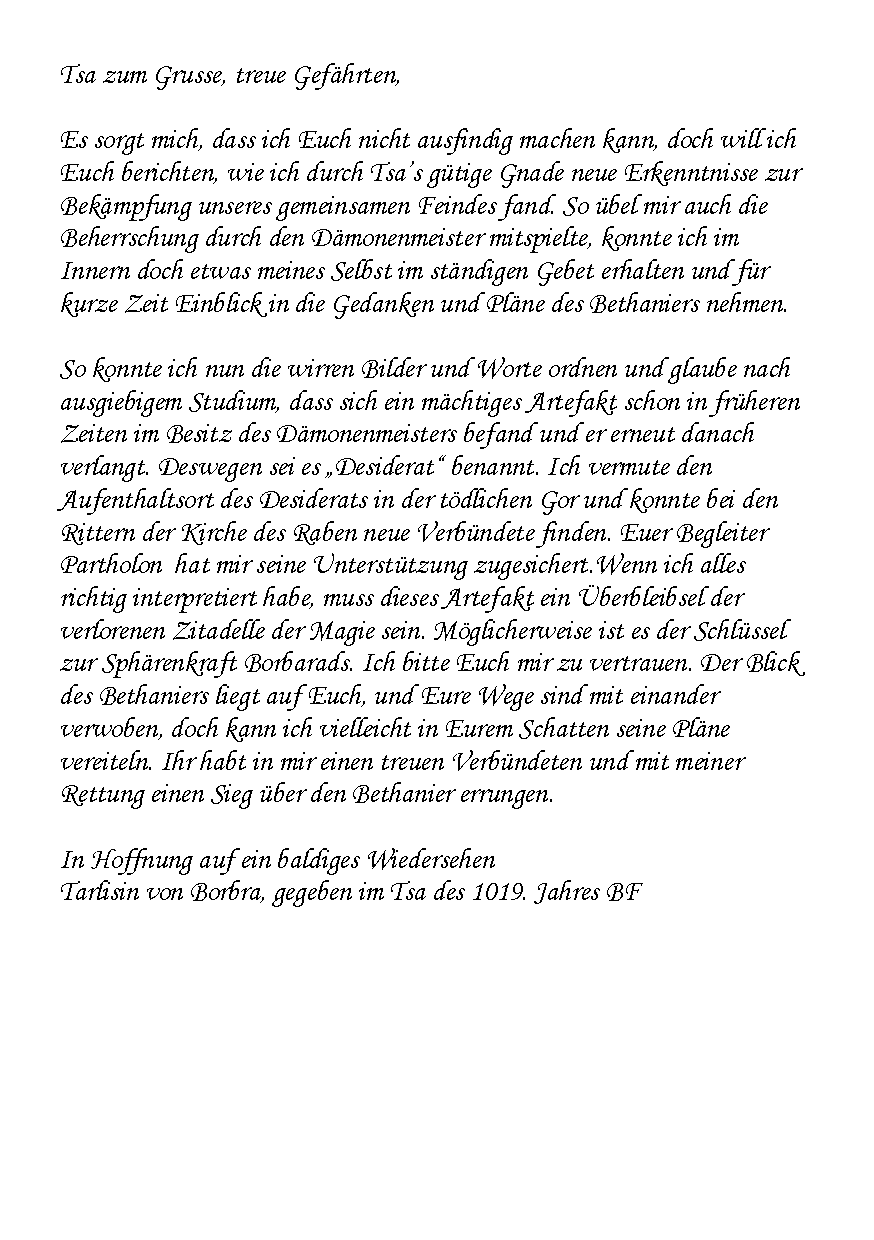
\includepdf[scale=0.9,pages=-]{handouts/part_3/gbabg_tarlisins_brief.pdf}
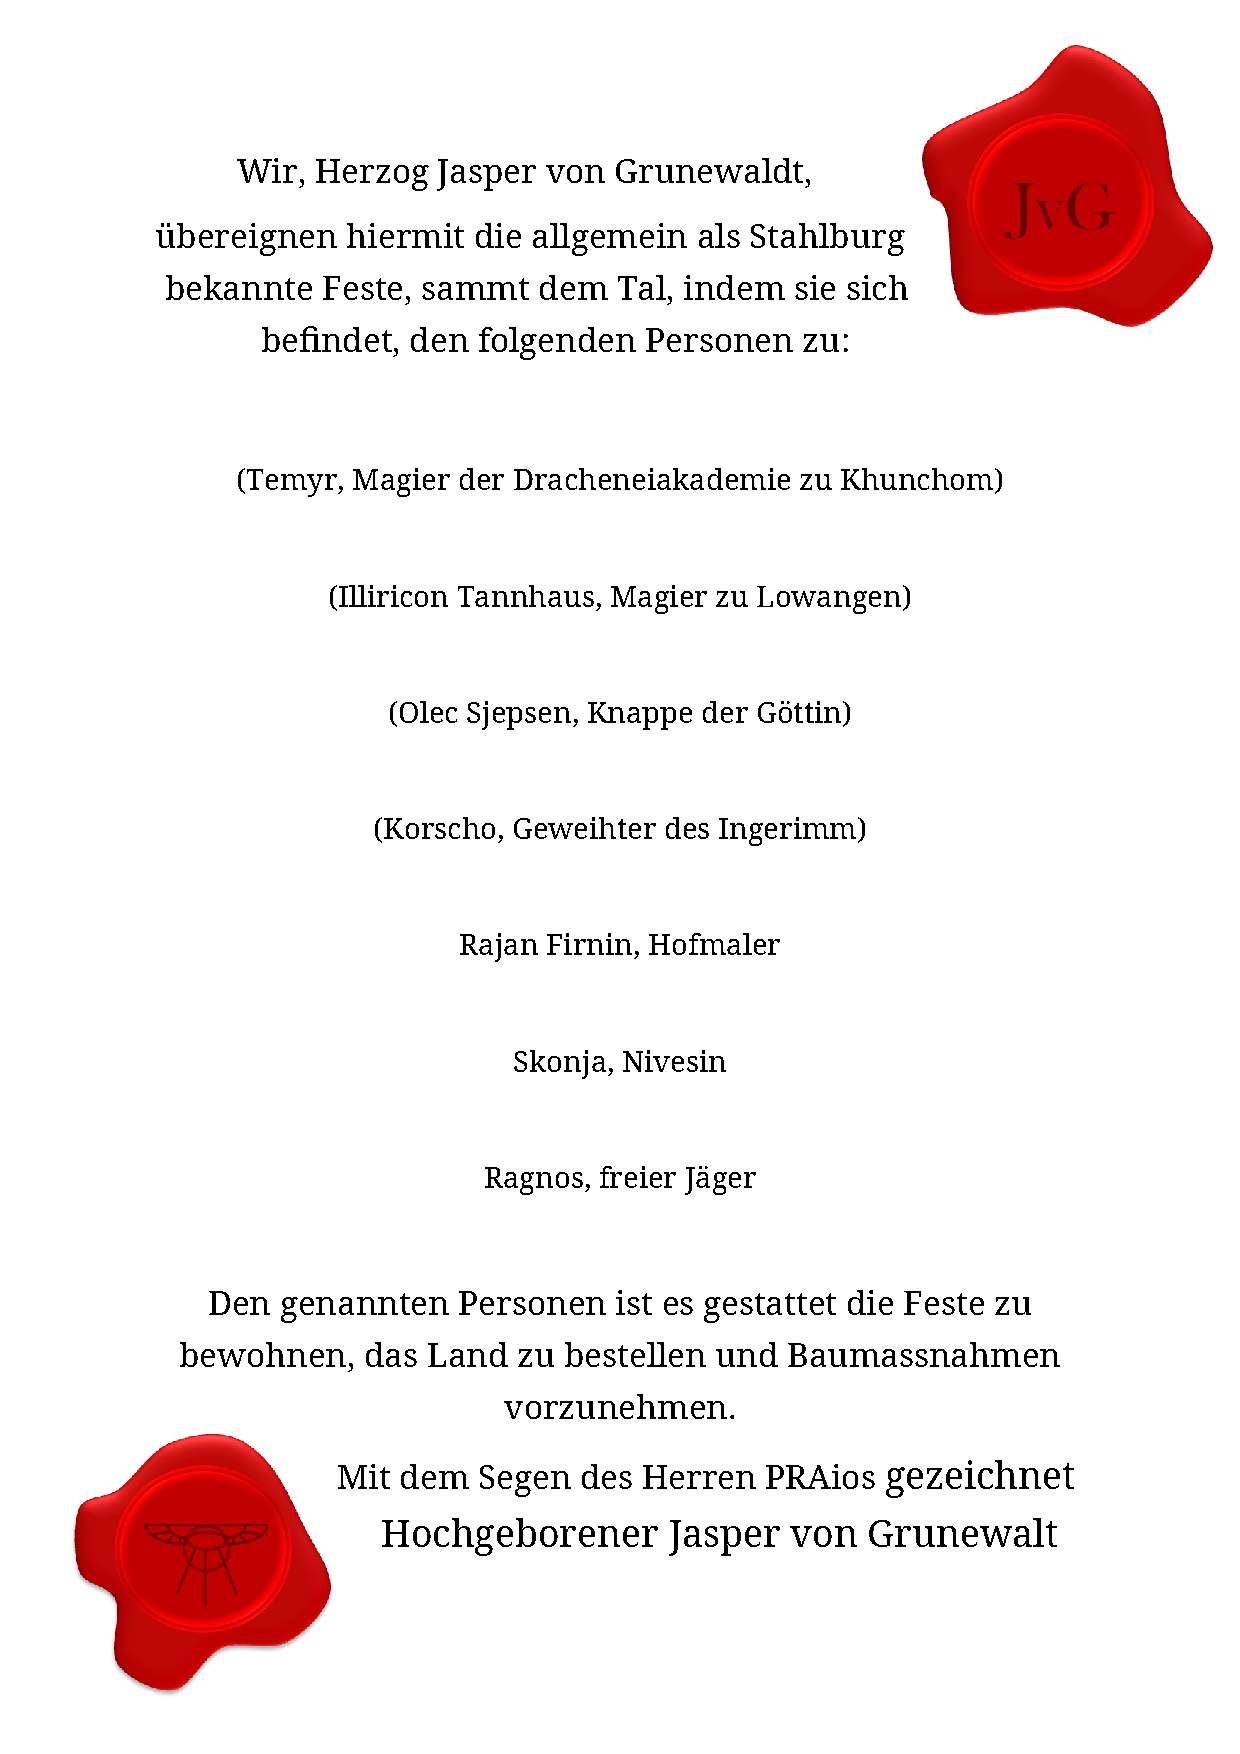
\includepdf[scale=0.9,pages=-]{handouts/part_3/Stahlburgurkunde.pdf}
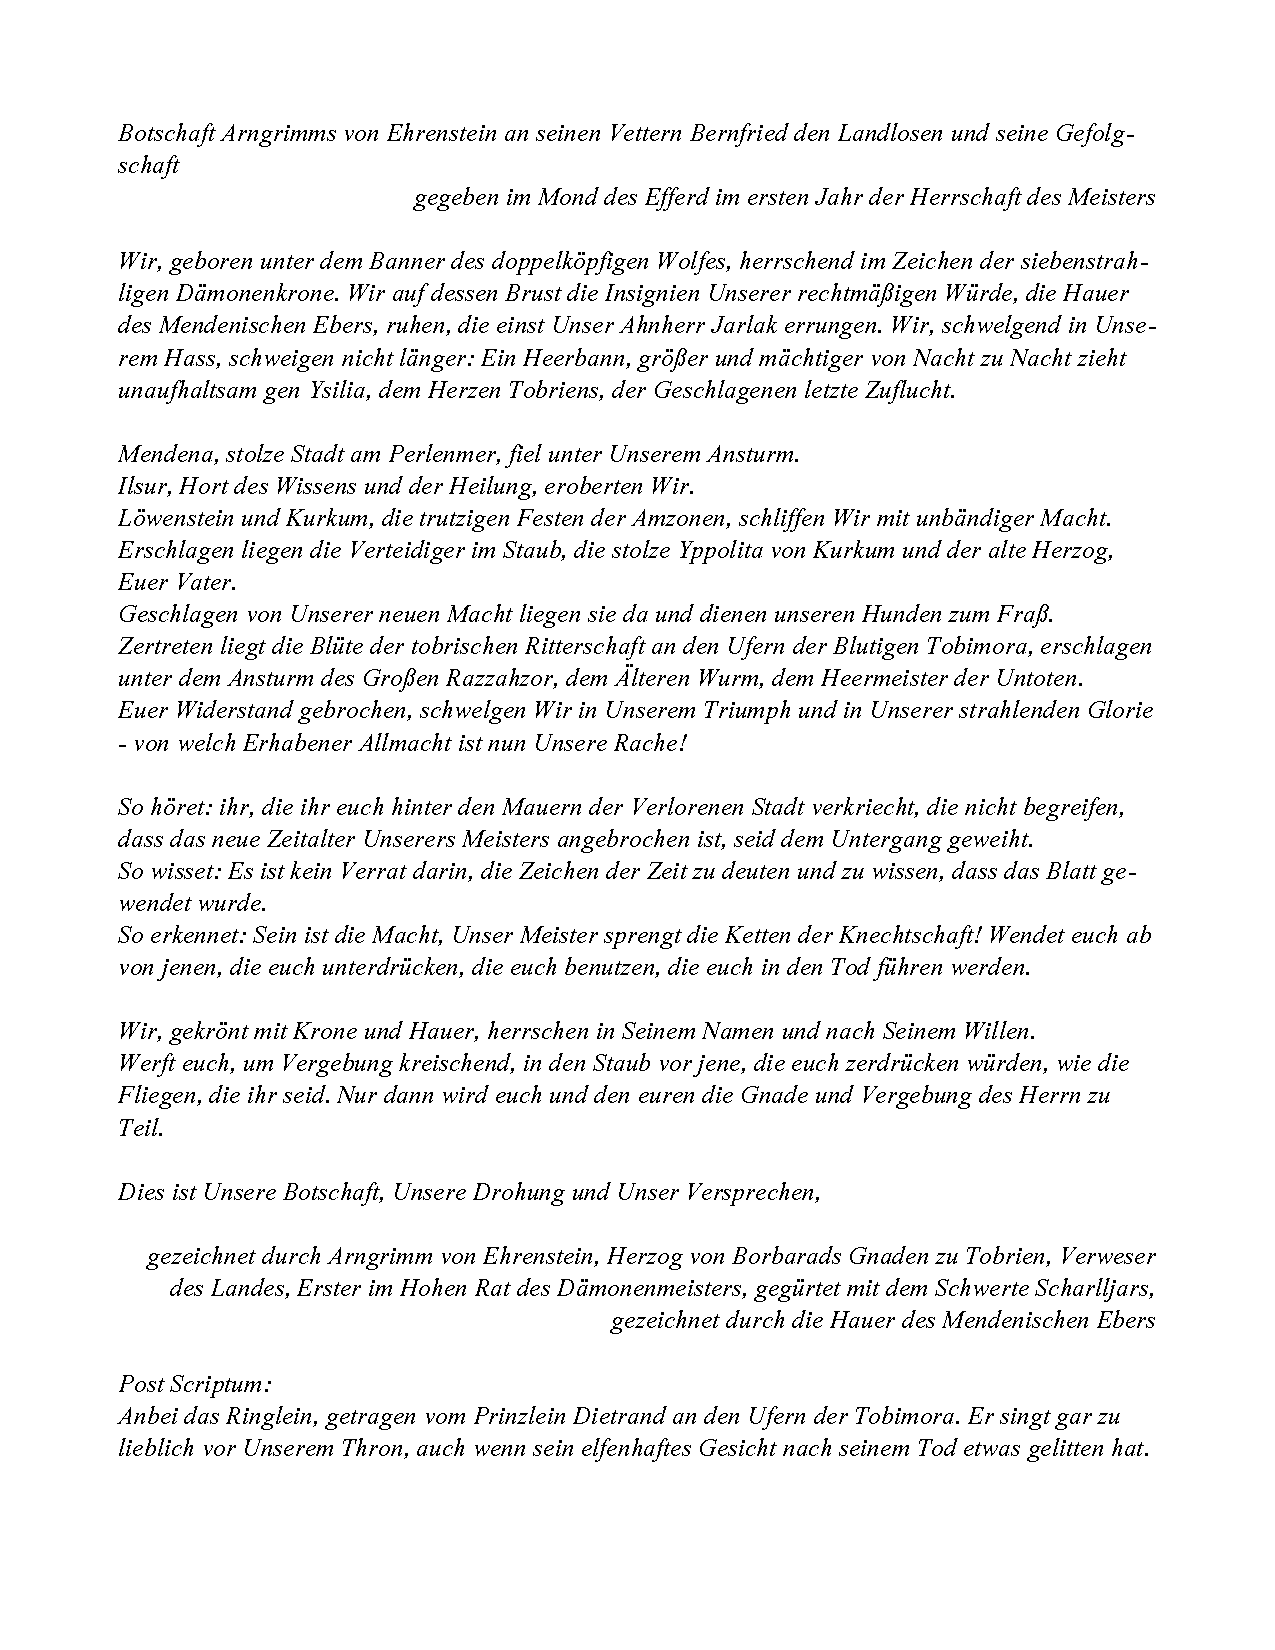
\includepdf[scale=0.9,pages=-]{handouts/part_3/wdw_botschaft_arngrimm.pdf}
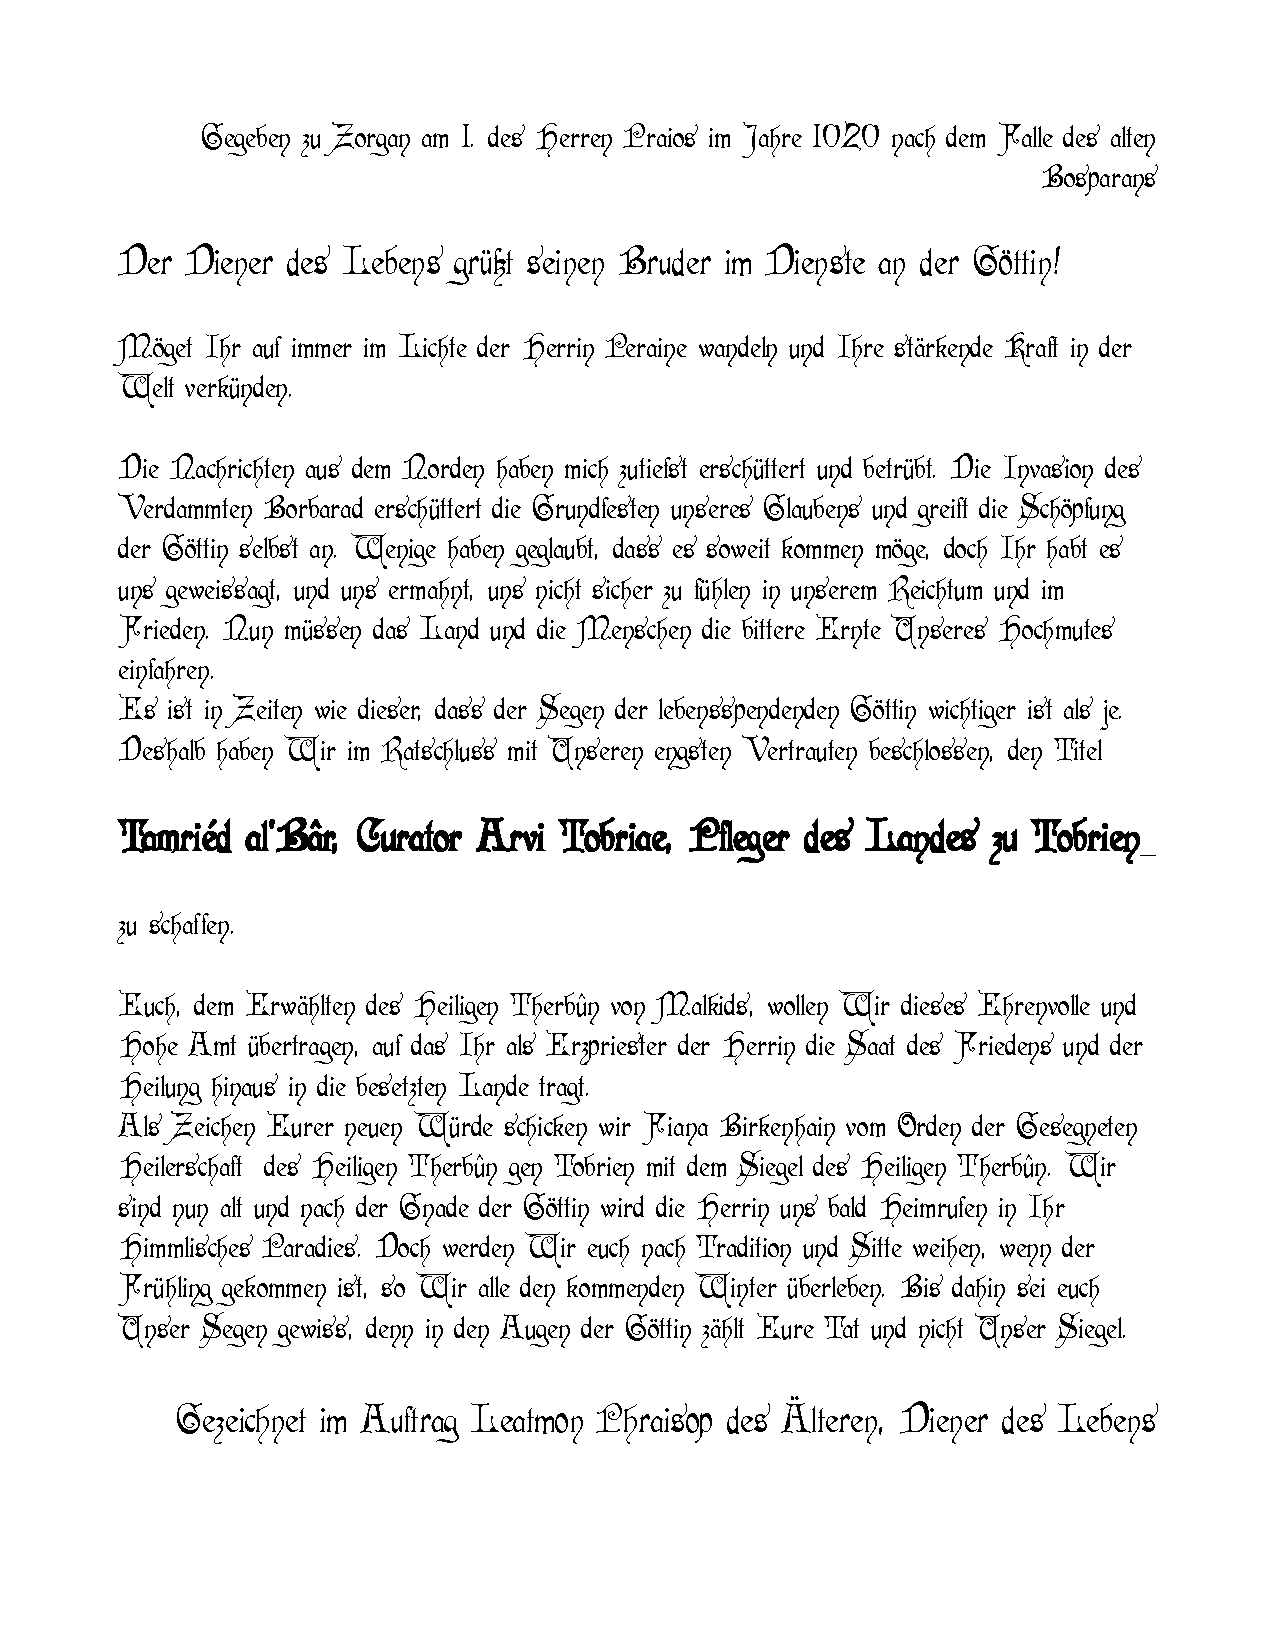
\includepdf[scale=0.9,pages=-]{handouts/part_3/wdw_brief_toran.pdf}
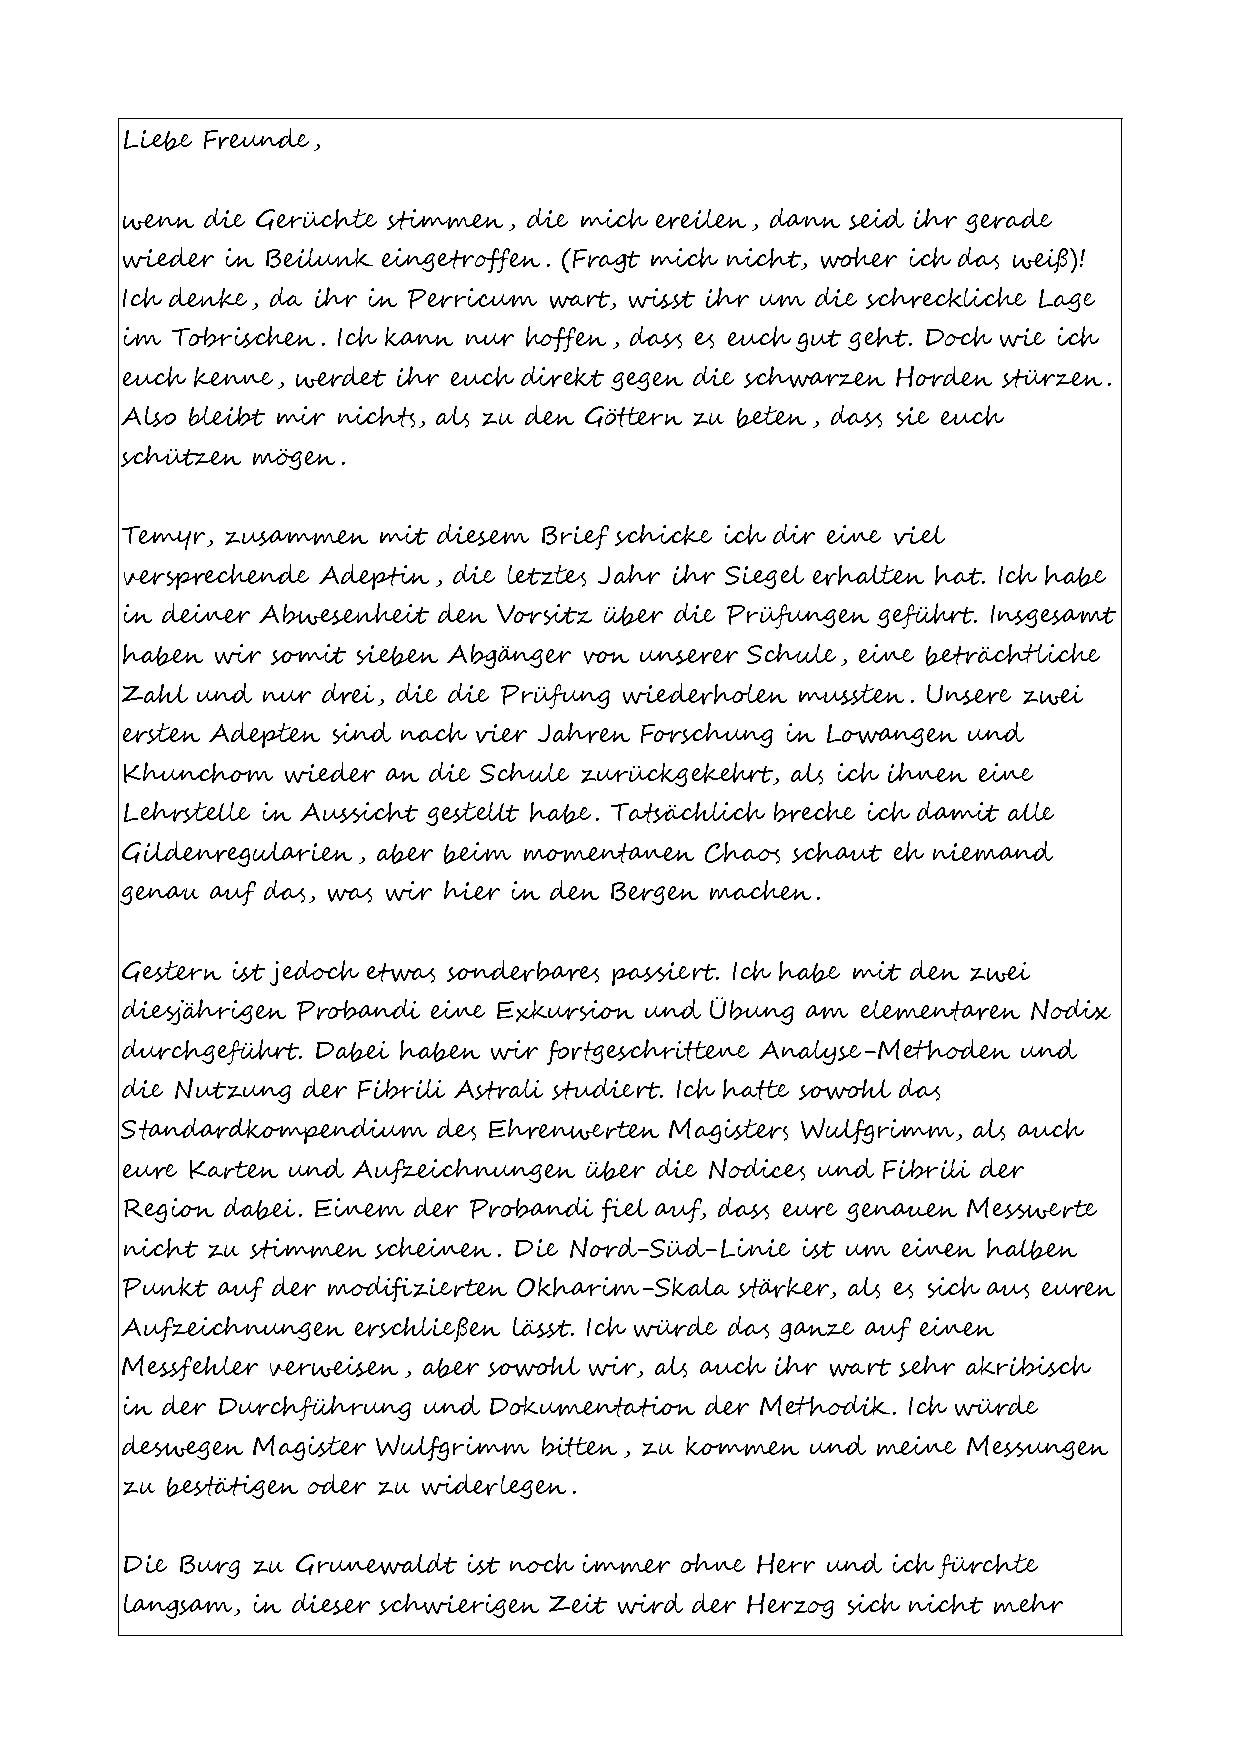
\includepdf[scale=0.9,pages=-]{handouts/part_3/wdw_brief_iliricon.pdf}